\chapter{Object detection and tracking using the Tensorflow API}

	\section{Object detection as Image Classification problem}
	\label{Object detection as Image Classification problem}
		Object detection is modeled as a classification problem. While classification is about predicting label of the object present in an image, detection goes further than that and finds locations of those objects too. In classification, it is assumed that object occupies a significant portion of the image.So it is about finding all the objects present in an image, predicting their labels/classes and assigning a bounding box around those objects.~\cite{objssd}
		
		In image classification, we predict the probabilities of each class, while in object detection, we also predict a bounding box containing the object of that class. So, the output of the network should be:
		\begin{itemize}
			\item Class probabilities (like classification)
			\item Bounding box coordinates. We denote these by cx(x coordinate of center), cy(y coordinate of center), h(height of object), w(width of object)
		\end{itemize}
		Class probabilities should also include one additional label representing background because a lot of locations in the image do not correspond to any object.
	
	\subsection{Sliding Window Detector}
		After the classification network is trained, it can then be used to carry out detection on a new image in a sliding window manner. First, we take a window of a certain size(blue box) and run it over the image at various locations. Then we crop the patches contained in the boxes and resize them to the input size of classification convnet. We then feed these patches into the network to obtain labels of the object. We repeat this process with smaller window size in order to be able to capture objects of smaller size. So the idea is that if there is an object present in an image, we would have a window that properly encompasses the object and produce label corresponding to that object.
	
	\subsection{Reducing redundant calculations}
		The following figure-6 shows an image of size 12 x 12 which is initially passed through 3 convolutional layers, each with filter size 3 × 3(with varying stride and max-pooling). Notice that, after passing through 3 convolutional layers, we are left with a feature map of size 3 x 3 x 64 which has been termed penultimate feature map i.e. feature map just before applying classification layer. We name this because we are going to be referring it repeatedly from here on. On top of this 3 x 3 map, we have applied a convolutional layer with a kernel of size 3 x 3. Three sets of this 3 x 3 filters are used here to obtain 3 class probabilities(for three classes) arranged in 1X1 feature map at the end of the network.
		
		\begin{figure}[htbp]
			\centering
			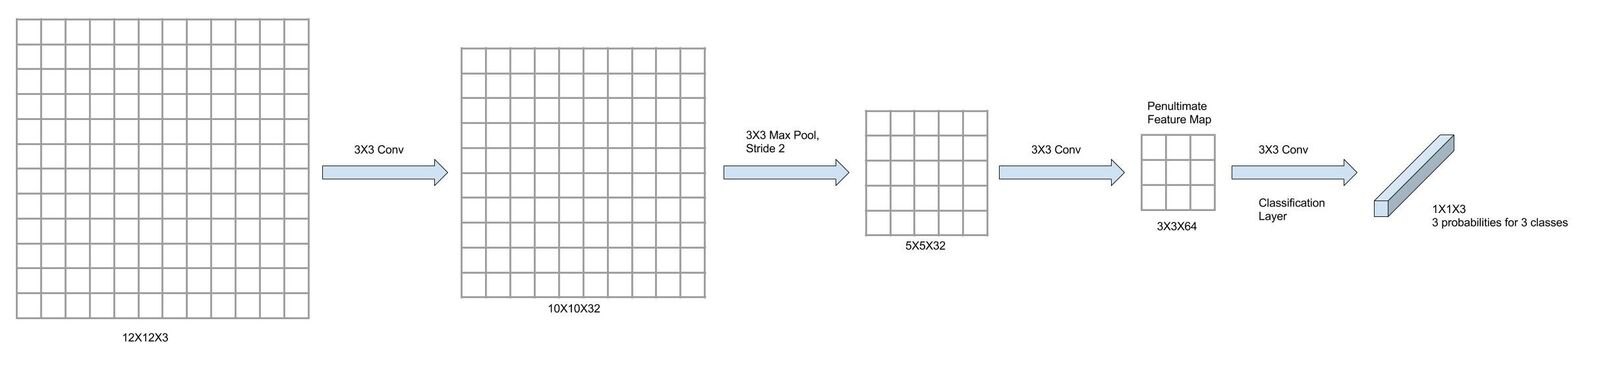
\includegraphics[width=16cm]{redun.jpg}
			\caption{Image of 12*12 passed through 3 conv layers\label{Image of 12*12 passed through 3 conv layers}}
		\end{figure}
	
		Now, we shall take a slightly bigger image to show a direct mapping between the input image and feature map. Let’s increase the image to 14 x 14. We can see that 12 x 12 patch in the top left quadrant(center at 6,6) is producing the 3×3 patch in penultimate layer colored in blue and finally giving 1×1 score in final feature map(colored in blue). The second patch of 12 x 12 size from the image located in top right quadrant(shown in red, center at 8,6) will correspondingly produce 1x1 score in final layer(marked in red).
		\begin{figure}[htbp]
			\centering
			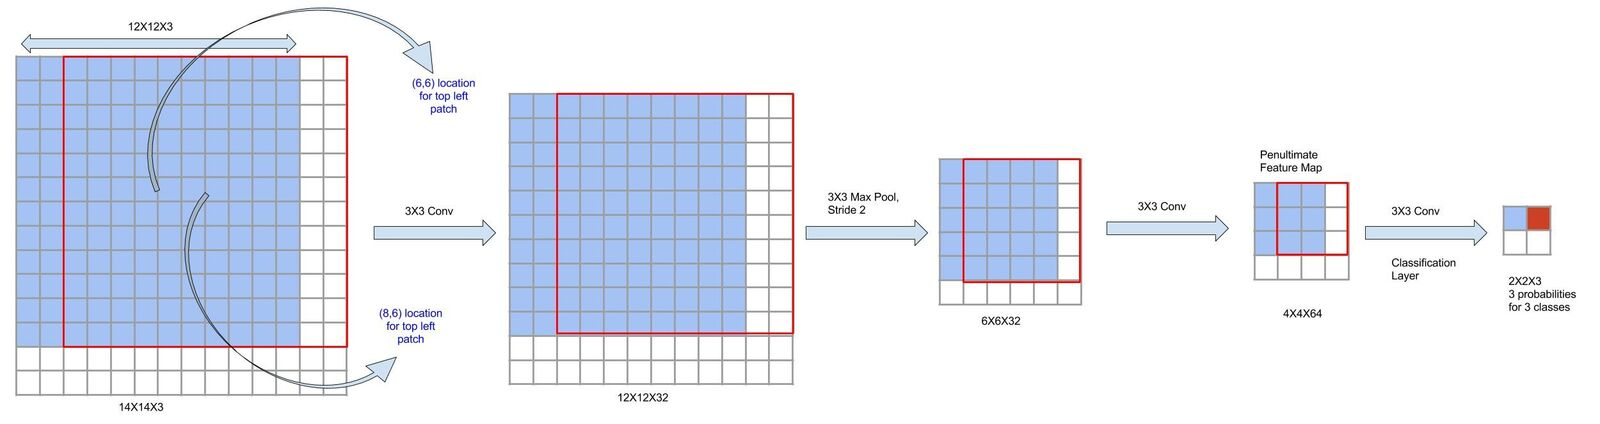
\includegraphics[width=16cm]{redun2.jpg}
			\caption{Depicting overlap in feature maps for overlapping image regions\label{Depicting overlap in feature maps for overlapping image regions}}
		\end{figure}
		
		To summarize we feed the whole image into the network at one go and obtain feature at the penultimate map. And then we run a sliding window detection with a 3 x 3 kernel convolution on top of this map to obtain class scores for different patches.
		
	\subsection{Training Methodology for modified network}
		\begin{figure}[htbp]
			\centering
			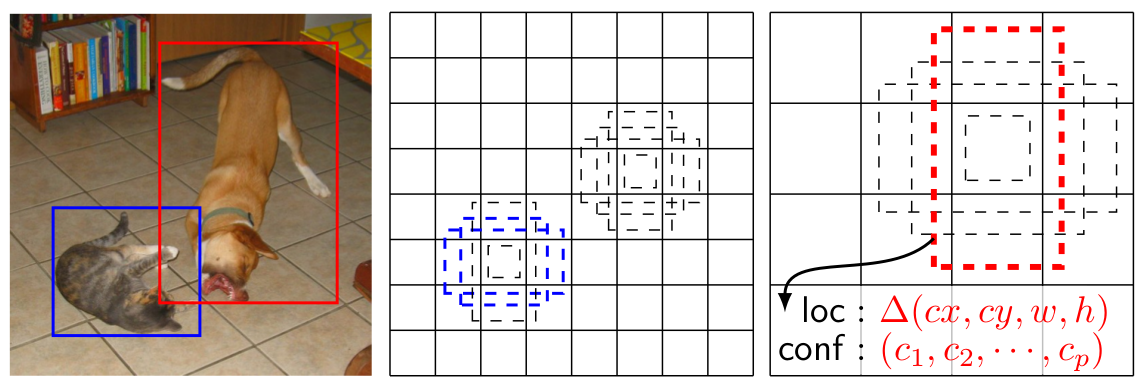
\includegraphics[width=16cm]{ssd2.png}
			\caption{Image with GT boxes, 8*8 feature map, 4*4 feature map\label{Image with GT boxes, 8*8 feature map, 4*4 feature map}}
		\end{figure}
		\newpage
		SSD~\cite{liu2016ssd} only needs an input image and ground truth boxes for each object during training. In a convolutional fashion, we evaluate a small set
		of default boxes of different aspect ratios at each location in several feature maps with different scales (e.g. 8*8 and 4*4 in the figures) For each default box, we predict both the shape offsets and the confidences for all object categories ($(c_1 , c_2 ,..., c_p)$).
		At training time, we first match these default boxes to the ground truth boxes. For example, we have matched two default boxes with the cat and one with the dog, which are treated as positives and the rest as negatives. The model loss is a weighted sum between localization loss (e.g. Smooth L1) and confidence loss (e.g. Softmax).
		
	\subsection{Working of the SSD Model}
		The SSD approach is based on a feed-forward convolutional network that produces a fixed-size collection of bounding boxes and scores for the presence of object class instances in those boxes, followed by a non-maximum suppression step to produce the final detections. The early network layers are based on a standard architecture used for high quality image classification (truncated before any classification layers).We then add auxiliary structure to the network to produce
		detections with the following key features:
		
		\begin{itemize}
			\item \emph{Multi-scale feature maps for detection:} We add convolutional feature layers to the end of the truncated base network. These layers decrease in size progressively and allow predictions of detections at multiple scales. The convolutional model for predicting detections is different for each feature layer (cf Overfeat and YOLO that operate on a single scale feature map).
			
			\item \emph{Convolutional predictors for detection:} Each added feature layer (or optionally an existing feature layer from the base network) can produce a fixed set of detection predictions using a set of convolutional filters. These are indicated on top of the SSD network architecture. The bounding box offset output values are measured relative to a default box position relative to each feature map location (cf the architecture of YOLO that
			uses an intermediate fully connected layer instead of a convolutional filter for this step).
			\begin{figure}[htbp]
				\centering
				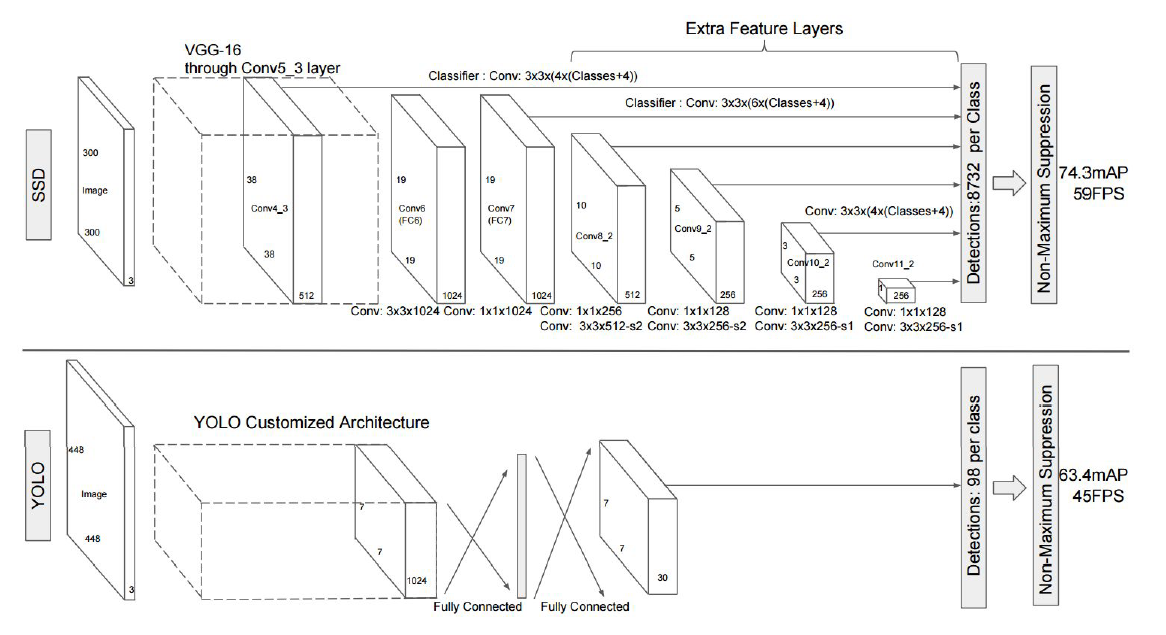
\includegraphics[width=16cm]{yolo-ssd.PNG}
				\caption{A comparison between two single shot detection models: SSD and YOLO\label{A comparison between two single shot detection models: SSD and YOLO}}
			\end{figure}
			
			\item \emph{Default boxes and aspect ratios"} We associate a set of default bounding boxes with each feature map cell, for multiple feature maps at the top of the network. The default boxes tile the feature map in a convolutional manner, so that the position of each box relative to its corresponding cell is fixed. Allowing different default box shapes in several feature maps let us efficiently discretize the space of possible output box shapes.
		\end{itemize}
		
		
	\section{Remote machine object detection node}
	\label{sec:Remote machine object detection node}
	
	\begin{figure}[htbp]
		\centering
		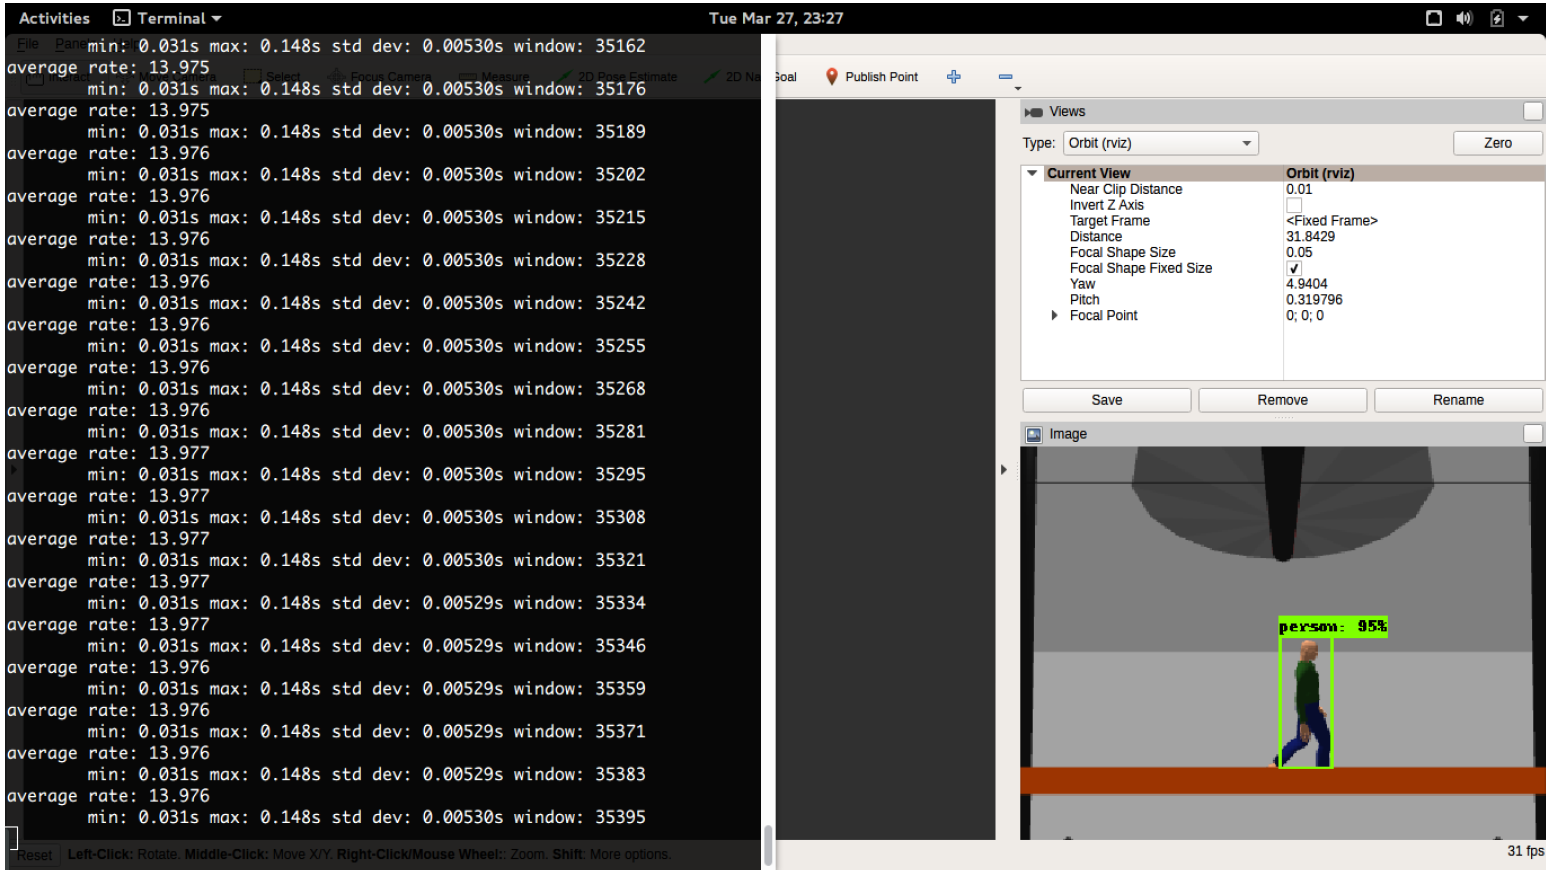
\includegraphics[width=12cm]{object_detection.PNG}
		\caption{Object detection along with rate on remote server\label{ROS working}}
	\end{figure}
	
	Deep Learning based approaches trained on the large datasets like Image-Net, such as SSD (Single Shot multi-box Detector)~\cite{liu2016ssd}, faster R-CNN ~\cite{ren2015faster}, YOLO (You Only Look
	Once) ~\cite{redmon2016you} etcetera have been consistently performing well for the classification of different objects, including humans. Detection is done using these methods in order to identify humans in the camera image from the drones. A simple comparison of the speed of the different methods leads to the top contenders, YOLO and SSD. Now, one of the big issues with these approaches, stopping them from real-time
	application in drones is the need of Graphical Processing Units (GPUs). These GPUs are heavy and power-hungry, thus cannot be placed on drones, also the smaller Nvidia Jetson boards have quite under-powered ARM based CPUs limiting small application as well.
	
	The solution that we propose is to use the Robot Operating System (ROS) in order to transfer the images captured to a separate computer on ground and then do the processing there and transfer the results back using the same architecture. This would allow us use huge computers with great computing power, which would then in turn allow us to use heavier and better performing techniques. This proposal
	will be limited by the bandwidth of the connection, as of now, this is being circumnavigated by sending images of smaller sizes. In order to further increase the rates of transfer we are only sending compressed images, which provide huge boosts to the processing rates (see table 5.1 for detailed time analysis).
	
	At present we are using the SSD, from the tensorflow object detection API ~\cite{tensorgit} released sometime back.
	
%	\begin{table}[h!]
%		\centering
%		\begin{tabular}{| c | c | c | c | c |}
%			\hline
%			Devices	& Image capture & Detection	& Transfer Uncompressed	& Compressed	\\ \hline  \hline
%			Intel i5-3250, No-GPU		& 34ms	& 130 ms	& NA	& NA\\ \hline
%			Nvidia GeForce 960M	& 34ms	& 60ms	& NA	& NA\\ \hline
%			Nvidia Titan X		& 34MS		& 5ms		& 500ms		& 10ms	\\ \hline
%		\end{tabular}
%		\caption{Time Analysis}
%		\label{table:Time Analysis}
%	\end{table}
	
	\section{Stereo image processing}
	\label{sec:Stereo image processing}
	
	\subsection{Stereo Image Capture}
		The  human  perception  of  depth  is  brought  about  by  the  hardly  understood  brain  process  of fusing  two  planar  images  obtained  from  slightly  different  perspective  viewpoints.  Due  to  the	different  viewpoint  of  each  eye,  a  small  horizontal  shift  exists,  called disparity,  between corresponding  image  points  in  the  left  and  right  view  images  on  the  retinas.  In  stereoscopic 
		vision, the objects to which the eyes are focused and accommodated have zero disparity, while objects  to  the  front  and  to  the  back  have  negative  and  positive  disparity,  respectively. The differences in disparity are interpreted by the brain as differences in depth ∆Z. 
		~\cite{lagendijk2002stereoscopic}
		\begin{figure}[htbp]
			\centering
			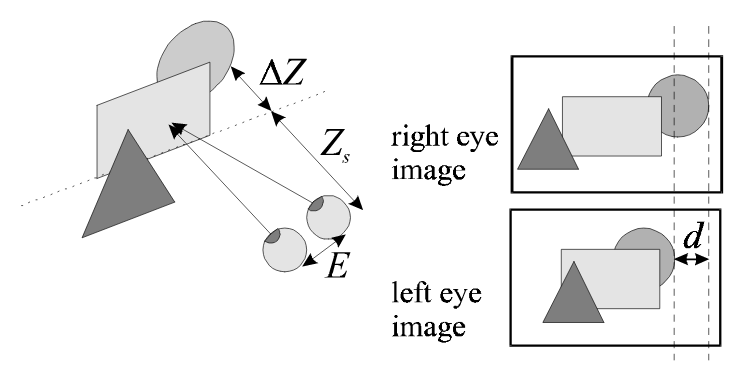
\includegraphics[width=12cm]{stereo2.png}
			\caption{Stereoscopic vision, resulting in different disparities depending on depth\label{Stereoscopic vision, resulting in different disparities depending on depth}}
		\end{figure}
		
		In order to be able to perceive depth using recorded images, a stereo camera (for eg. Zed Camera) is required which  consists  of  two  cameras  that  capture  two  different,  horizontally  shifted  perspective viewpoints.  This  results  in  a  shift  (or disparity)  of  objects  in  the  recorded  scene  between  the left  and  the  right  view  depending  on  their  depth.  In  most  cases  the  interaxial separation or baseline B between  the  two  lenses  of  the  stereoscopic  camera  is  in  the  same  order  as  the  eye distance E (6  to  8  cm).  In  a  simple  camera  model  the  optical  axes  are  assumed  to  be  parallel. The depth Z and disparity d are then related as follows:
		\begin{equation}
		d = \lambda \frac{B}{\lambda - Z}
		\end{equation}
		
		where $\lambda$ is the focal length of the cameras. A  more  complicated  camera  model  takes  into  account  the convergence  of  the  camera  axes  with  angle $\beta$. The  disparity  is  not  only dependent  on  the  depth Z of  an  object,  but  also  on  the  horizontal  object  position X. Furthermore,   a   converging   camera configuration   also   leads   to   small   vertical   disparity components,  which  are,  however,  often  ignored  in  subsequent  processing  of  the  stereoscopic data.
		
		When  recording  stereoscopic  image  sequences,  the  camera  setup  should  be  such  that,  when displaying the stereoscopic images, the resulting shifts between corresponding points in the left and right view images on the display screen allow for comfortable viewing. If the observer is at a distance $Z_s$ from the screen, then the observed depth $Z_{obs}$ and displayed disparity d are related as:
		\begin{equation}
		Z_{obs} = Z_s \frac{E}{E-d}
		\end{equation}
		
		In  the  case  that  the  camera  position  and  focusing  are  changing dynamically,  as  is  the  case  for  instance in stereoscopic television production where the stereo camera may be zooming, the camera geometry is controlled by a set of production rules. If the recorded images are to be used  for  multiviewpoint  stereoscopic  display,  a  larger  interaxial  lens  separation  needs  to  be used,  sometimes  even  up  to  1  meter.  In  any  case  the  camera  setup  should  be  geometrically calibrated  such  that  the  two  cameras  capture  the  same  part  of  the  real  world  scene. 
	
	\newpage
	\subsection{Disparity Estimation}
		The  key  difference  between  planar  and  stereoscopic  images  and  image  sequences  is  that  the latter  implicitly  contains  depth  information  in  the  form  of  disparity  between  the  left  and  right view images. Not only is the presence of disparity information essential to the ability of humans to  perceive  depth,  disparity  can  also  be  exploited  for  automated  depth  segmentation  of  real world   scenes,   and   for   compression   and   interpolation   of   stereoscopic   images   or   image sequences.
		\begin{figure}[htbp]
			\centering
			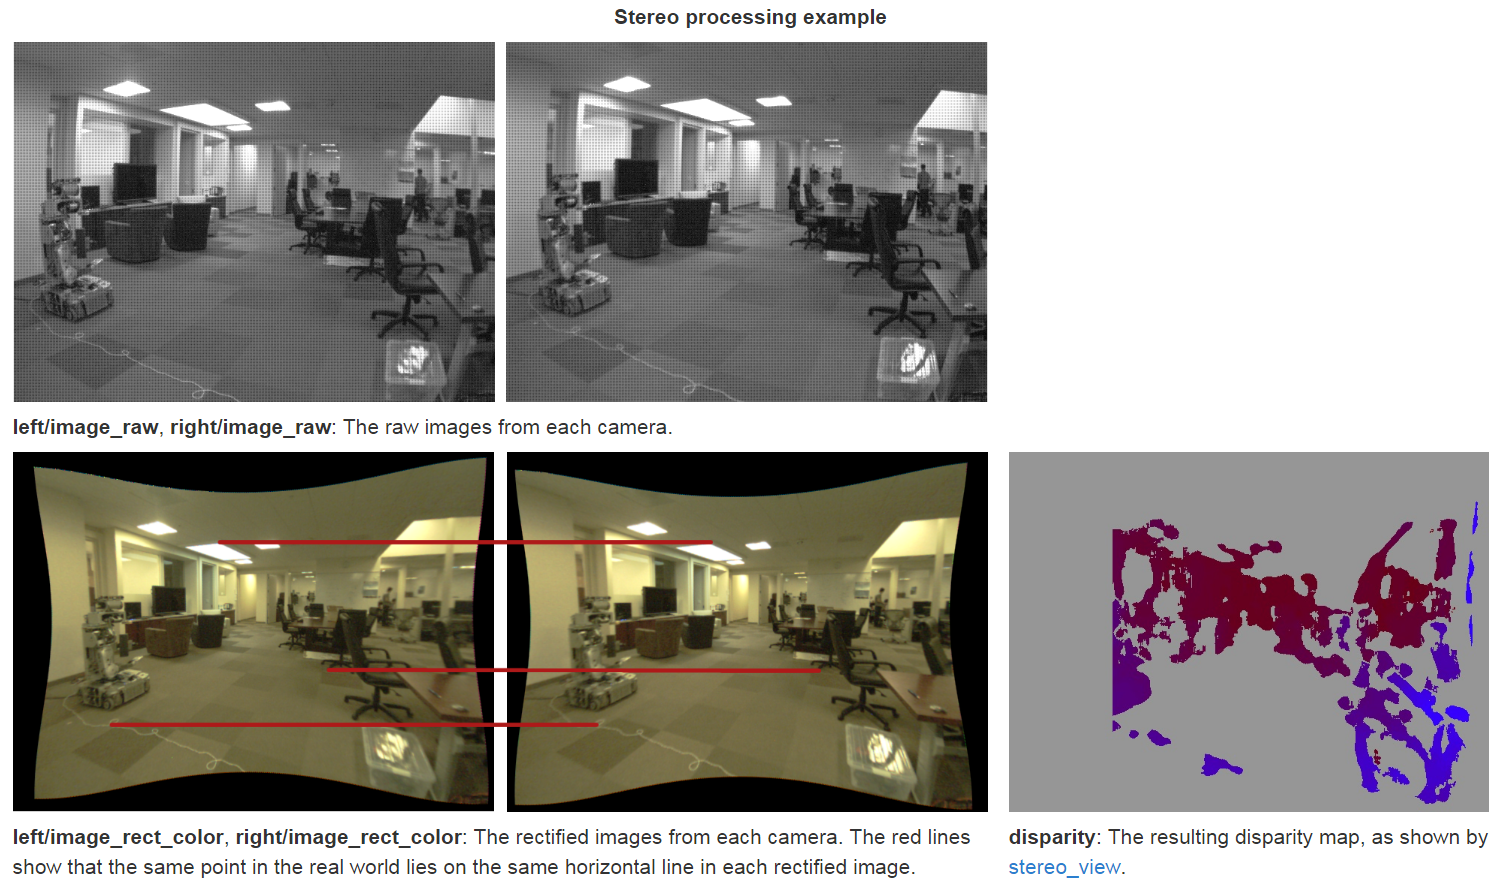
\includegraphics[width=16cm]{disparity.PNG}
			\caption{Disparity field in the stereo image pair \label{Disparity field in the stereo image pair }}
		\end{figure}
		
		Disparity estimation is essentially a correspondence problem. The correspondence between the two  images  can  be  determined  by  either  matching  features  or  by  operating  on  or  matching  of small patches of gray values. Feature matching requires as a preprocessing step the extraction of appropriate features from the images, such as object edges and corners. After obtaining the features,  the  correspondence  problem  is  first  solved  for  the  spatial  locations  at  which  the features  occur,  from  which  next  the  full  disparity field  can  be  deduced  by  for  instance interpolation  or  segmentation  procedures.  Feature-based  disparity  estimation  is  especially 
		useful in the analysis of scenes for robot vision applications.
		\begin{figure}[htbp]
			\centering
			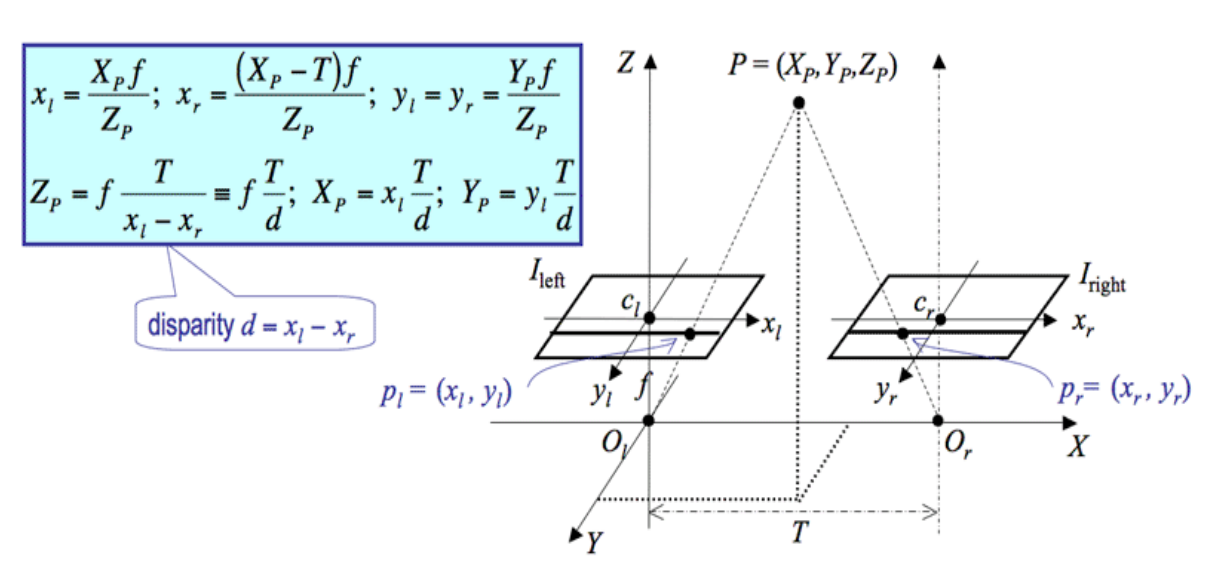
\includegraphics[width=16cm]{stereo3.png}
			\caption{Disparity calculation \label{Disparity calculation }}
		\end{figure}
		
		Most  disparity  estimation  algorithms  used  in  stereoscopic  communications  rely  on  matching small  patches  of  gray  values  from  one  view  to  the  gray  values  in  the  alternate  view.  The matching  of  this  small  patch  is  not  carried  out  in  the  entire  alternate  image,  but  only  within  a relatively  small  search  region  to  limit  the  computational  complexity.  Standard  methods typically  use  a  rectangular  match  block  of  relatively  small  size  (e.g.,  8x8  pixels). The relative horizontal shift between a match block and the block within the search region  of  the  alternate  image  that  results  in  the  smallest  value  of  a  criterion  function  used,  is then  assigned  as  disparity  vector  to  the  center  of  that  match  block.  Often  used  criterion 
		functions are the sum of squares and the sum of the absolutes values of the differences between the  gray  values  in  the  match  block  and  the  block  being  considered  in  the  search  region.
		
		In  image  analysis  problems,  disparity  estimation  is  often  considered  in  combination  with  the segmentation   of   the   stereoscopic   image   pair.   Joint   disparity   estimation   and   texture segmentation   methods   partition   the   image   pair   into   spatially   homogeneous   regions   of approximately  equal  depth.  Disparity  estimation  in  image  sequences  is  typically  carried  out independently  on  successive  frame  pairs.  Nevertheless,  the  need  for  temporal  consistency  of successive   disparity   fields   often   requires   temporal   dependencies   to   be   exploited   by postprocessing  of  the  disparity  fields.  If  an  image  sequence  is  recorded  as  an  interlaced  video  
		signal,  disparity  estimation  should  be  carried  out  on  the  individual  fields instead  of  frames  to avoid confusion between motion displacements and disparity.
	
	
	\subsection{Working module}
	
	Stereo images acquired from the simulation were used to calculate a disparity map, by making use of relative positions of the camera. The specs of the simulated camera are shown in table 5.2. The disparity of features between two stereo images are usually computed as a shift to the left of an image feature when viewed in the right image. In real world applications since stereo images may not always be correctly aligned to
	allow for quick disparity calculation, images obtained are first rectified for the relative rotations of the cameras. After rectification, the correspondence problem can be solved using an algorithm that scans both the left and right images for matching image features to compute disparity by the normalized correlation.
	
	\begin{equation}NC = \frac{\sum\sum L(r,c).R(r,c-d)}{\sqrt{(\sum\sum L(r,c)^2).(\sum\sum R(r,c-d)^2)}}\end{equation}
	
	We make use of the "stereo image proc" package in ROS to calculate and publish the normalized correlation disparity.
	
	\begin{table}[h!]
		\centering
		\begin{tabular}{| c | c |}
			\hline
			\textbf{Quantity}	& \textbf{Value}	\\ \hline  \hline
			Image Resolution		& 400x400	\\ \hline
			$h_{fov}$	& 80 degrees	\\ \hline
			baseline		& 20 cm		\\ \hline
			Update rate	& 30 Hz		\\ \hline
		\end{tabular}
		\caption{Stereo Camera Specifications}
		\label{table:Stereo Camera Specifications}
	\end{table}
	
	
	\newpage
	\section{Distance estimation}
	\label{sec:Distance estimation}
	
	\subsection{Using Stereo camera images}
	Using disparity image calculated from stereo image matching as well as the object bounding box obtained from the detection node, we estimate the distance of the object from the camera. From the bounding box region extracted from
	the disparity image, the largest cluster of similar-valued pixels is extracted and identified to be the cluster belonging to the human. A mean value of the pixels belonging to this cluster is calculated, which is used to obtain the depth
	estimate by the image projection formulae
	\begin{equation}z = \frac{f.T}{V}\end{equation}
	
	where z is the distance to be estimated, d is the disparity value, f is the focal length of the camera in pixels and T is the baseline in real world units.
	\begin{figure}[htbp]
		\centering
		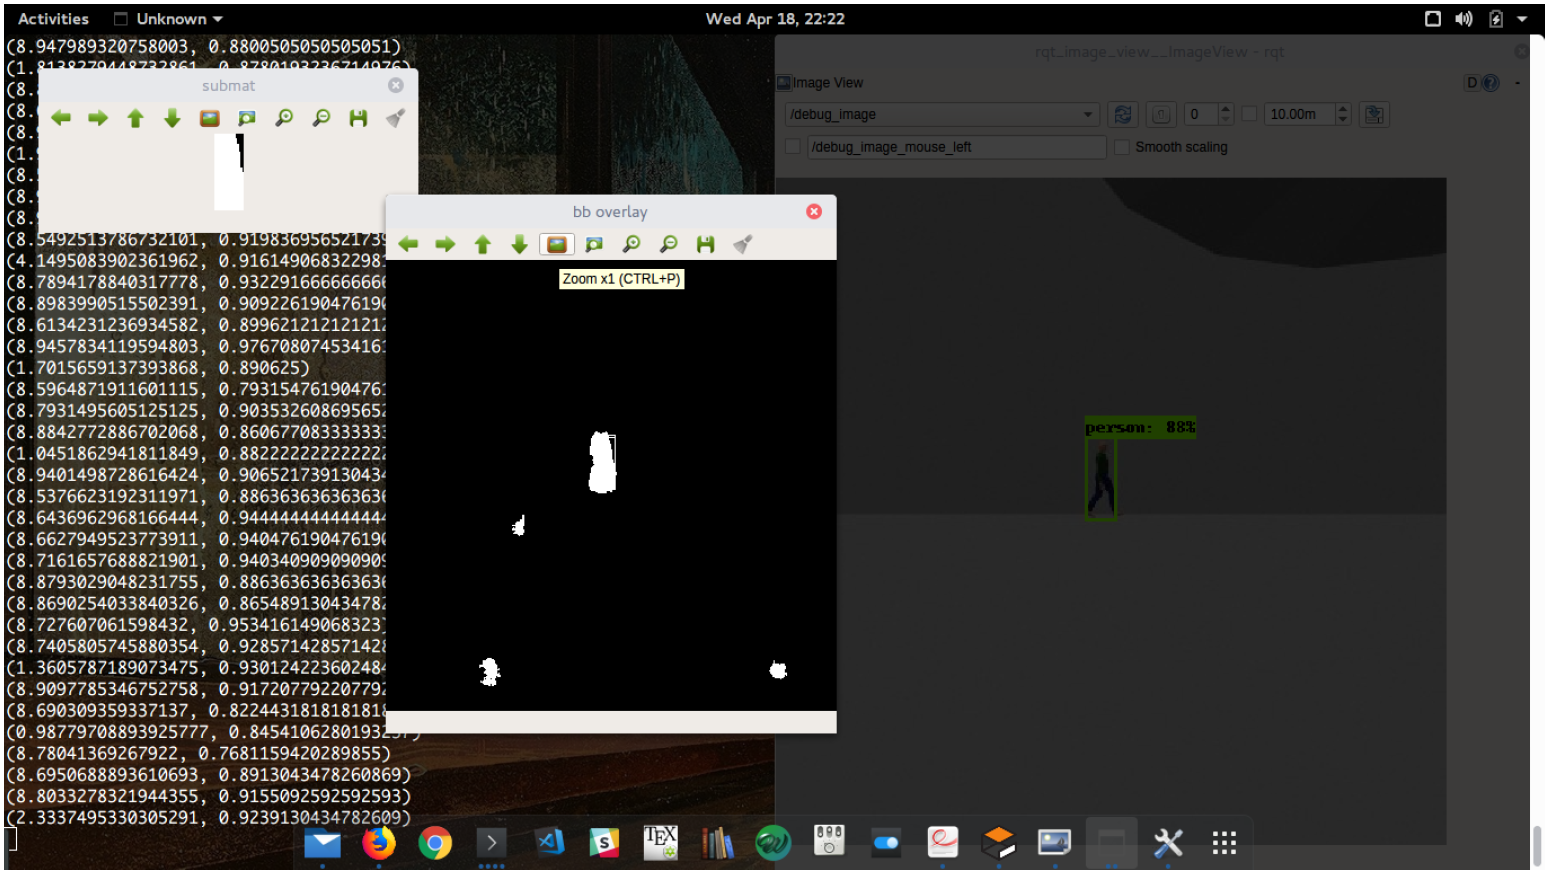
\includegraphics[width=16cm]{disparity_map.png}
		\caption{Distance estimation results \label{Distance estimation results}}
	\end{figure}
	
	\subsection{Using ORB features from monocular camera image}
	Another monocular camera based approach was developed for depth estimation in the project, using the scaling factors obtained from measuring the spread of ORB features in the image. The algorithm proposed was as follows
	
	\begin{itemize}
		\item Detect ORB features in the image
		\item Remove features lying outside bounding box for the image
		\item match the features in consecutive images and remove unmatched features
		\item calculate std. deviation of the features in x and y for
		both t and t+1 image frames
		\item obtain estimates of rate of change of depth using
		aspect ratio of bounding boxes
		\item remove the estimate (x or y) with greater change
		from previous value
	\end{itemize}
	
	\begin{figure}[htbp]
		\centering
		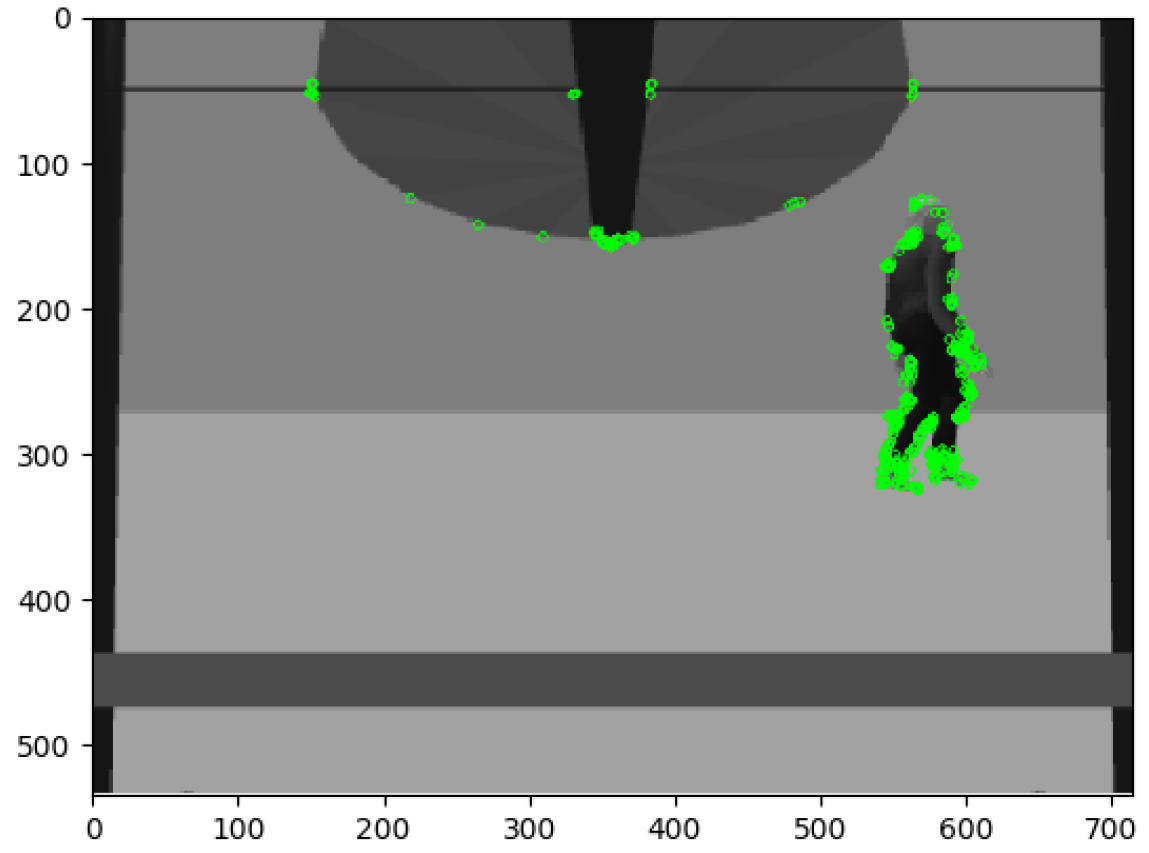
\includegraphics[width=12cm]{orb_features.PNG}
		\caption{ORB features in image frame\label{ROS working}}
	\end{figure}
	
	The algorithm makes use of the fact that change in depth of an object from camera is inversely proportional to its visible size in the image and directly proportional to the true size of the object. Hence,
	\begin{equation}\delta{z} = k.l(\frac{1}{x}_{t} - \frac{1}{x}_{t+1}) \end{equation}
	
	where $\delta{z}$ is the change in true depth of the object, ${x}_{t}$ ,${x}_{t+1}$ are sizes of projection in images at t and t+1 frames, l is the true size of object and k is proportionality constant. We estimate the size of the object in the image by the std deviation of the ORB features inside the bounding box in the image. Since this value is susceptible to changes by occlusion, we use the true size of the visible portion as the true size of the object in the formulae. Also adding the assumption the the object will be either occluded in x direction or y direction at a time,
	
	\begin{equation}\delta{z}_{x} = k.(w/L)(\frac{1}{std^{t}}_{x} - \frac{1}{std^{t+1}}_{x}) \end{equation}
	\begin{equation}\delta{z}_{y} = k.(l/W)(\frac{1}{std^{t}}_{y} - \frac{1}{std^{t+1}}_{y}) \end{equation}
	
	where w,l are true sizes of visible portions and W,L are total true sizes of the objects. Hence, quantities \emph{w/L}, \emph{l/W} can be estimated by aspect ratio and its inverse of the smaller bounding box in the images.
	
	Finally, the stereo method was chosen since it gave more
	robust depth estimates.
	
	\begin{figure}[htb]
		\centering
		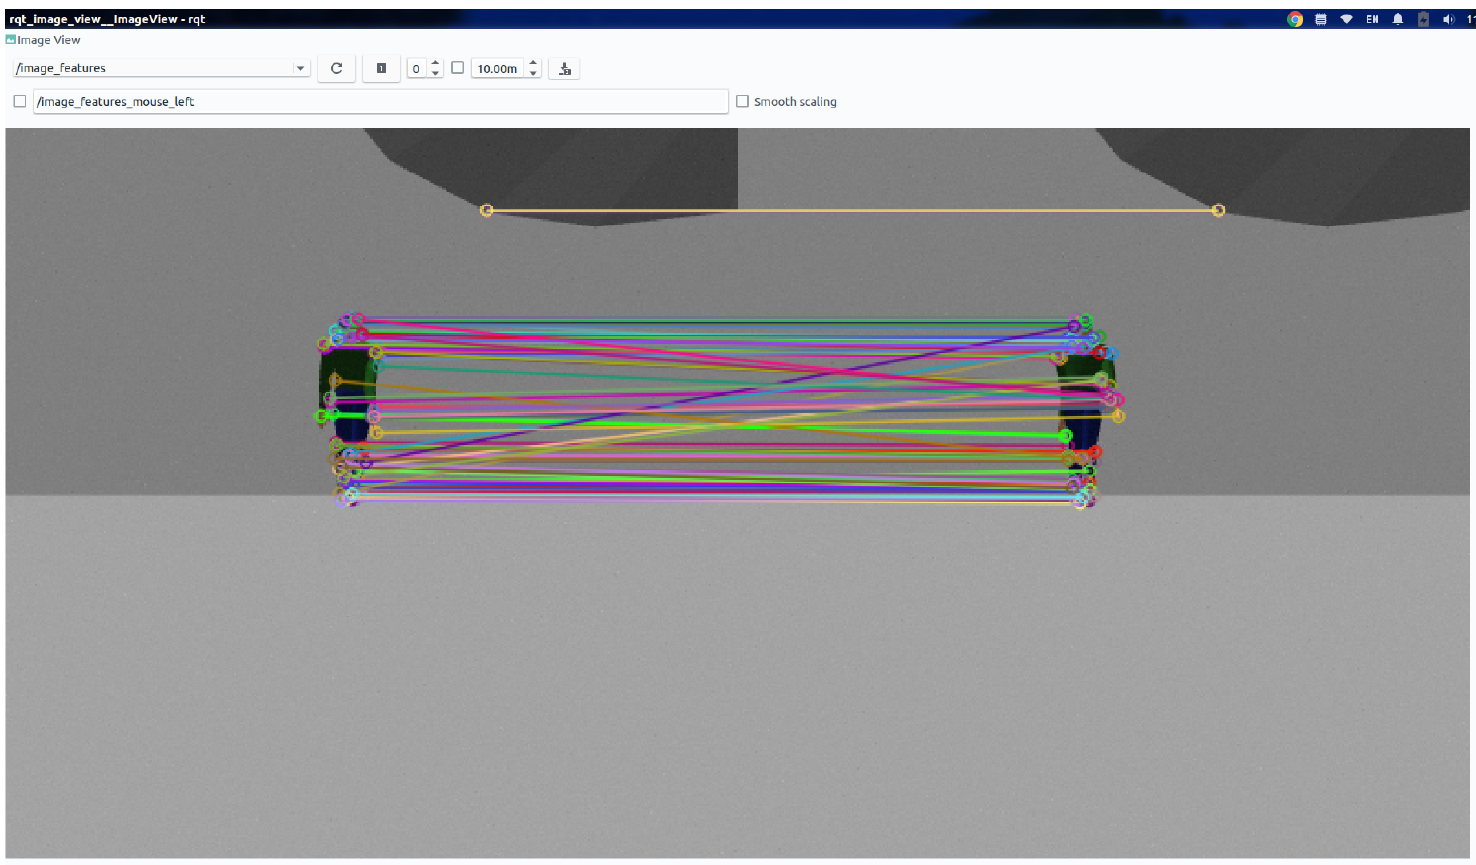
\includegraphics[width=12cm]{matched_orb_features.PNG}
		\caption{Matched ORB features in consecutive frames\label{Matched ORB features in consecutive frames}}
	\end{figure}
	
	
	\section{Kalman Filtering}
	\label{sec:Kalman Filtering}
	The  Kalman  filter  uses  a  prediction  followed  by  a  correction  in  order  to  determine  the  states  of the  filter~\cite{rhudy2017kalman}. This  is  sometimes  called  predictor-corrector, or  prediction-update. The  main  idea  is that using information about the dynamics of the state, the filter will project forward and predict what  the  next  state  will  be. This  can  be  thought  of  as  a  numerical  integration  technique  such  as  Euler’s method   or   Runge-Kutta. The   correction   or   update   part   then   involves   comparing   a measurement with what we predict that measurement should be based on our predicted states. 
	The  Kalman  filtering  technique  is  now  discussed  in  equation  format.    Starting  from  some  initial state  estimate, $\hat{x}_0$,  and  initial  state  error  covariance  matrix, $P_0$,  the  predictor-corrector  format  is applied  recursively  at  each  time  step,  e.g.  using  a  loop. First,  the  state  vector  is  predicted  from the state dynamic equation using 
	\begin{equation}
	\hat{x}_{k|k-1} = F_{k-1}\hat{x}_{k-1} + G_{k-1}u_{k-1}
	\end{equation}
	
	where $\hat{x}_{k|k-1}$ is the predicted state vector,$\hat{x}_{k-1}$ is the previous estimated state vector, $u$ is the input vector, and $F$ and $G$
	are matrices defining the system dynamics. The subscript $k|k-1$ is read as “$k$ given $k-1$” and is a shorthand notation for the state at discrete time
	$k$ given its previous  state  at  discrete  time $k-1$,  i.e.  this  is  the  prediction  of  the  state  using  the  system  model projected forward one step in time.  Next, the state error covariance matrix must also be predicted using 
	\begin{equation}
	P_{k|k-1} = F_{k-1}P_{k-1}F^{T}_{k-1} + Q_{k-1}
	\end{equation}
	
	where $P_{k|k-1}$ represents  the  predicted  state  error  covariance  matrix, 
	$P_{k-1}$ is  the  previous  estimated 
	state  error  covariance  matrix,  and $Q$ is  the  process  noise  covariance  matrix. Again,$k|k-1$  is indicating  that  this  is  the  expected  covariance  matrix  at $k$ based  on  the  system  model  and  the covariance  at $k-1$.    Once  the  predicted  values  are  obtained,  the  Kalman  gain  matrix,$K_k$, is 
	calculated by 
	\begin{equation}
	K_k = P_{k|k-1}H^{T}_k(H_kP_{k|k-1}H^T_k + R_k)^{-1}
	\end{equation}
	where $H$is  a  matrix  necessary  to  define  the  output  equation  and $R$ is  the  measurement  noise covariance.  The state vector is then updated by scaling the “innovation,” which is the difference between  the  measurement  of  the  output, $z_k$,  and  the  predicted  output, $H_k\hat{x}_{k|k-1}$(sometimes 
	called $\hat{y}_{k|k-1}$),  by  the  calculated  Kalman  gain  matrix  in  order  to  correct  the  prediction  by  the appropriate amount, as in 
	\begin{equation}
	\hat{x}_k = \hat{x}_{k|k-1} + K_k(z_k - H_k\hat{x}_{k|k-1})
	\end{equation}
	Similarly, the state error covariance is updated by
	\begin{equation}
	P_k = (I - K_kH_k)P_{k|k-1}
	\end{equation}
	where $I$ is an identity matrix. 
	
	The estimates of bounding box coordinates obtained from object detection node, as well as the depth estimates obtained from stereo-disparity images and rate of change of depth estimation from ORB features were combined to be fed as measurements for the relative state of the object(human) in pixel coordinates into the kalman filter. The Kalman filter, running at 30 Hz, was employed to smooth out the obtained measurements as well as provide predictions in case the measurement generating nodes failed to provide any measurement. Furthermore, the predictive capability of the kalman filter was also leveraged to provide measurements in case the object to be tracked was occluded, since the measurements will not be generated in such cases as well.
	
	A vanilla Kalman filter can be modelled as
	\begin{equation}
	\begin{aligned}
	x_0 = Gaussian(\mu_0,\Sigma_0) \\
	x_{t+1} = A_t.x_t + b_t + \epsilon^{1}_{t+1} \\
	y_{t} = C_t.x_t + d_t + \epsilon^{2}_{t} \\
	\epsilon^{1}_{t} = Gaussian(0,Q) \\
	\epsilon^{2}_{t} = Gaussian(0,R) \\
	\end{aligned}
	\end{equation}

	where x is the model state and y are the measurements.
	For our case
	\begin{equation}
	\begin{aligned}
	x_t
	=\begin{bmatrix}
	x_c \\ y_c \\ z_c \\ v_x \\ v_y \\ v_z \\a_x \\a_y \\a_z
	\end{bmatrix}
	&
	y_t
	=\begin{bmatrix}
	x_m \\ y_m \\ z_m \\ v_z
	\end{bmatrix}
	\end{aligned}
	\end{equation}
			
	The state-transition and observation matrices for tracking human subject
	\begin{equation}
	A_t=
	\begin{bmatrix}
		1 & 0 & 0 & T & 0 & 0 & 0.5*T^2 & 0 & 0\\
		0 & 1 & 0 & 0 & T & 0 & 0 & 0.5*T^2 & 0\\
		0 & 0 & 1 & 0 & 0 & T & 0 & 0 & 0.5*T^2\\
		0 & 0 & 0 & 1 & 0 & 0 & T & 0 & 0\\
		0 & 0 & 0 & 0 & 1 & 0 & 0 & T & 0\\
		0 & 0 & 0 & 0 & 0 & 1 & 0 & 0 & T\\
		0 & 0 & 0 & 0 & 0 & 0 & 1 & 0 & 0\\
		0 & 0 & 0 & 0 & 0 & 0 & 0 & 1 & 0\\
		0 & 0 & 0 & 0 & 0 & 0 & 0 & 0 & 1
	\end{bmatrix}
	\end{equation}
	\begin{equation}
	C_t =
	\begin{bmatrix}
		1 & 0 & 0 & 0 & 0 & 0 & 0 & 0 & 0\\
		0 & 1 & 0 & 0 & 0 & 0 & 0 & 0 & 0\\
		0 & 0 & 1 & 0 & 0 & 0 & 0 & 0 & 0\\
		0 & 0 & 0 & 0 & 0 & 1 & 0 & 0 & 0\\
	\end{bmatrix}
	\end{equation}
	
	with $b_t$ and $d_t$ set to 0.
	
	Values of process and measurement noise parameters Q and R are determined from measurement set using Expectation-Maximization, which is a way to find
	maximum-likelihood estimates for model parameters when your data is incomplete, has missing data points, or has unobserved (hidden) latent variables. It is an iterative way to approximate the maximum likelihood function. It works by choosing random values for the missing data points, and using those guesses to estimate a second set of data. The new values are used to create a better guess for the first set, and the process continues until the algorithm converges on
	a fixed point. The EM algorithm:
	\begin{equation}Q(\theta|\theta^{t}) = E_{Z|X, \theta^{t}}(logL(Z,X,\theta))\end{equation}
	\begin{equation}\theta^{t+1} = argmax_{\theta}Q(\theta|\theta^{t})\end{equation}
	
	Where measurements modelled as X and Z is the latent variable over which distributions are formed. The values of noise parameters (modelled by $\theta$) are estimated during the 2nd step (M-step).
	
	\newpage
	\section{Object of interest tracking}
	\label{sec:Object of interest tracking}

	The implementation of this project in the real world would certainly command the need to use wireless networks for information exchange between the ground based server and the quadrotor. Now, the prime options for communication
	of this kind would be 4G/5G mobile networks or WiFi, give the short range of WiFi, for long range applications one would move towards the former option. One of the biggest issues which we anticipate this method would have to deal with, would be the occasional frame drop when transferring image data at high rate. In order to deal with this we use a ROS implementation of ”High Speed Tracking with Kernelized Correlation Filter” ~\cite{henriques2015high}. Our implementation is based off of code from Tomas Vojir.~\cite{kcf}
	
	Given an initial image patch containing the target, the goal is to learn a classifier to discriminate between its appearance and that of the environment. This classifier can be evaluated exhaustively  at  many  locations,  in  order  to  detect  it  in
	subsequent frames. Of course, each new detection provides a new image patch that can be used to update the model.
	
	it  is  tempting  to  focus  on  characterizing  the  object  of
	interest  –  the  positive  samples  for  the  classifier.  However,
	a  core  tenet  of  discriminative  methods  is  to  give  as  much
	importance,  or  more,  to  the  relevant  environment  –  the
	negative samples. The most commonly used negative samples are image patches from different locations and scales,
	reflecting  the  prior  knowledge  that  the  classifier  will  be
	evaluated under those conditions.
	
	An  extremely  challenging  factor  is  the  virtually  unlimited amount of negative samples that can be obtained from
	an  image.  Due  to  the  time-sensitive  nature  of  tracking,
	modern  trackers  walk  a  fine  line  between  incorporating
	as  many  samples  as  possible  and  keeping  computational
	demand low. It is common practice to randomly choose only
	a few samples each frame.
	
	Here we use tools to analytically incorporate thousands of samples at different relative translations, without iterating over them
	explicitly. This is made possible by the discovery that, in the
	Fourier domain, some learning algorithms actually become
	easier as we add more samples, if we use a specific model for translations.
	These  analytical  tools,  namely  circulant  matrices,  provide  a  useful  bridge  between  popular  learning  algorithms
	and  classical  signal  processing. This tracker is based  on  Kernel  Ridge  Re-
	gression  that  does  not  suffer  from  the  “curse  of  ker-
	nelization”,  which  is  its  larger  asymptotic  complexity,  and
	even  exhibits  lower  complexity  than  unstructured  linear
	regression.  Instead,  it  can  be  seen  as  a  kernelized  version
	of  a  linear  correlation  filter,  which  forms  the  basis  for  the
	fastest  trackers  available.  The  powerful  kernel  trick is leveraged at  the  same  computational  complexity  as
	linear correlation filters.
	
	\subsection{Fast Kernel Correlation}
	
	Even though there are faster algorithms for training and detection, they still rely on computing one kernel correlation each ($k^{xx}$ and $k^{xz}$ respectively). The kernel
	correlation consists of computing the kernel for all relative shifts of two input vectors. This represents the last standing computational bottleneck, as a naive evaluation of n  kernels for signals of size n will have quadratic complexity. However, using the cyclic shift model will allow us to efficiently exploit the redundancies in this expensive computation.
	
	
	KCF kernel
	\begin{equation}k_{xx^{'}} = exp(-\frac{1}{\sigma^2}(||x||^2+||x^{'}||^2-2F^{-1}(\tilde{x}.\tilde{x^{'}})))\end{equation}
	
	Where $x$ and $x^{'}$ are image patches being compared. This computation can be performed in O(nlog(n)).
	
	The idea behind this method is that given one (or more) labels one should be able to perform online learning in order to discriminate between patches of interest and the background. More details on the original implementation can be easily found. Now since this is a very less computationally involved, the rate of performance goes as up as high as 100 frames per second. This lets us relax up the condition on the detection pipeline. As for the first labeled frame, we have used the detection bounding box returned after the execution of first frame.
	
	With an interestingly symmetric argument, training with multiple base samples and a single channel can be done in the  primal,  with  only  element-wise  operations. This  follows  by  applying  the  same  reasoning  to  the non-centered covariance matrix XTX, instead of XXT. In this case we obtain the original MOSSE filter. For  fast  element-wise  operations  we  can
	choose multiple channels (in the dual, obtaining the DCF) or multiple base samples (in the primal, obtaining the MOSSE), but not both at the same time. This has an important impact on  time-critical  applications,  such  as  tracking. The  general case is  much  more  expensive  and  suitable  mostly  for offline training applications.
	
	\begin{figure}[htb]
		\centering
		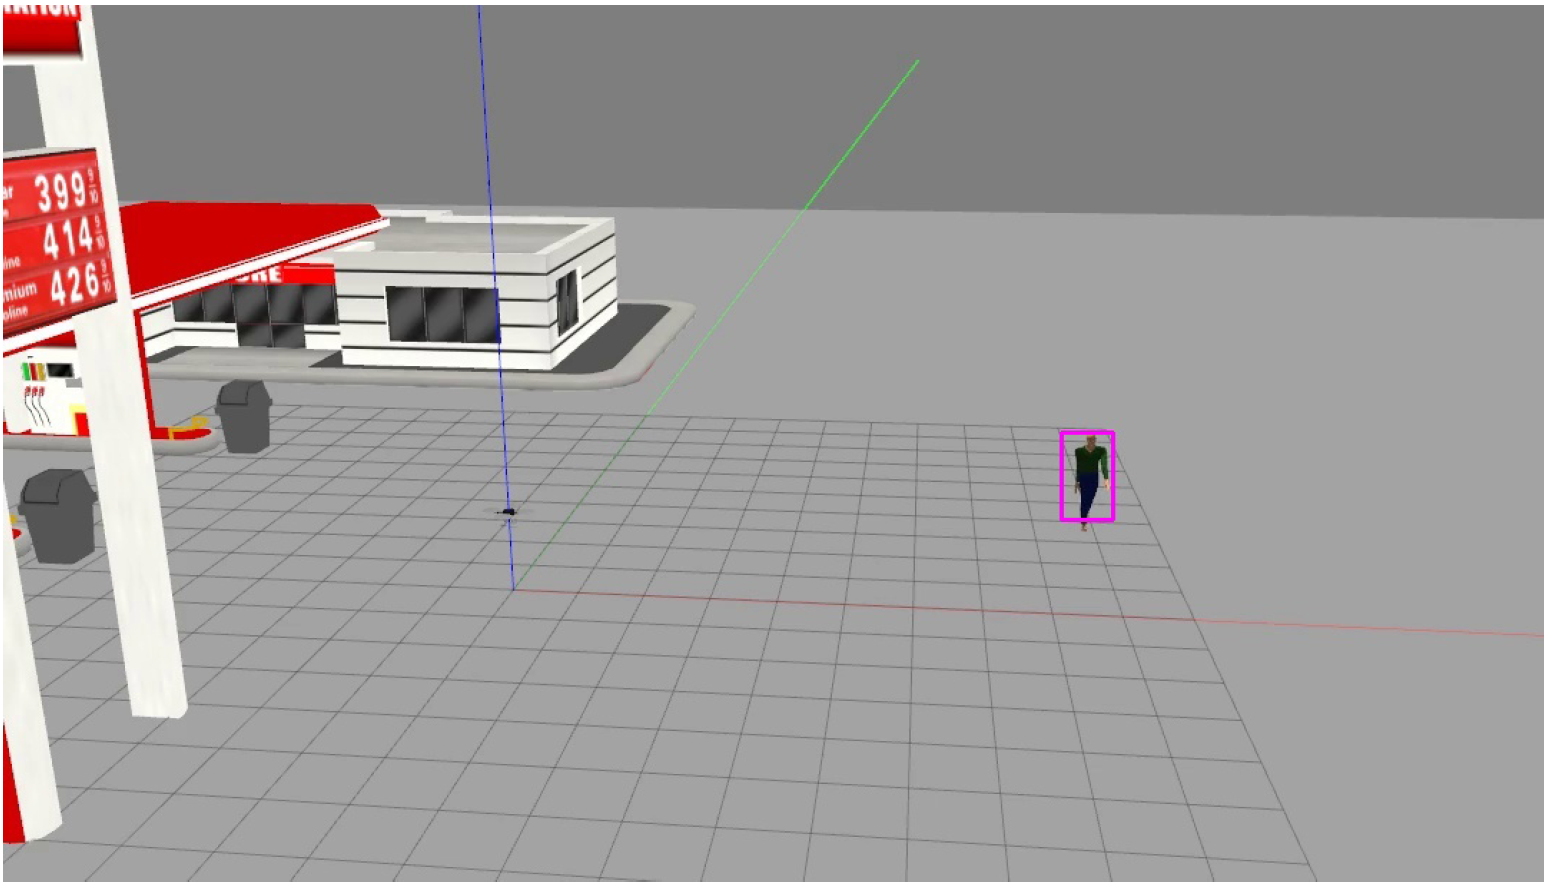
\includegraphics[width=16cm]{KCF_tracked.PNG}
		\caption{KCF Tracked human subject\label{KCF Tracked human subject}}
	\end{figure}
	
	
	
	